\graphicspath{ {./figures/metabolism/} }

%%%%%%%%%%%%%%%%%%$%%%%%%%%%%%%%%%%%

\section{Supporting figures}

\begin{figure}[h!]
\centering
\includegraphics[scale=1.0]{./figure_S1a}
\captionsetup{width=.65\linewidth}
\caption[Block diagram depiction of the mathematical model.]{\textbf{Block diagram depiction of the mathematical model.} Boxes contain transfer functions relating upstream and downstream variables, open circles indicate summation points. Transfer functions are expressed in the Laplace frequency domain.}
\label{fig:metabolism:figS1a}
\end{figure}

\begin{figure}[h!]
\centering
\includegraphics[scale=1.0]{./figure_S1b}
\caption[Error frequencies are broadly increased when an auxiliary repressor is lost.]{\textbf{Error frequencies are broadly increased when an auxiliary repressor is lost.} (A,B) Simulations were performed with 2500 independent parameter sets quasi-randomly sampled from the nine-dimensional hyperspace defined by one order of magnitude variation in each of the model parameters. (A) Error frequencies are projected onto two dimensional planes and then linearly interpolated onto (100 px)\textsuperscript{2} grids. (B) Binned counts of the 2500 simulated error frequencies depicted in A. The majority of parameter sets yield high error frequencies.}
\label{fig:metabolism:figS1b}
\end{figure}

\begin{figure}[h!]
\centering
\includegraphics[scale=1.0]{./figure_S1c}
\captionsetup{width=.65\linewidth}
\caption[Error frequencies increase when a repressor is lost irrespective of where the success threshold is set.]{\textbf{Error frequencies increase when a repressor is lost irrespective of where the success threshold is set.} Error frequencies for parameter sets from Fig. \ref{fig:metabolism:figS1b} were re-calculated across a range of different success thresholds. Thresholds are defined by the 99\textsuperscript{th} percentile of protein levels simulated with all repressors, and are evaluated at the time when the mean protein level with all repressors reaches the indicated fraction of its maximum value. Each line represents one of the parameter sets from Fig. \ref{fig:metabolism:figS1b}. Color scale reflects maximum difference in error frequency across the range of thresholds tested.}
\label{fig:metabolism:figS1c}
\end{figure}

\begin{figure}[h!]
\centering
\includegraphics[width=1.0\columnwidth]{./figure_S2a}
\caption[Reduced energy metabolism diminishes the importance of auxiliary repressors over a wide range of model conditions.]{\textbf{Reduced energy metabolism diminishes the importance of auxiliary repressors over a wide range of model conditions.} (A-G) For each panel, 2500 simulations were performed with parameter sets quasi-randomly sampled from the nine-dimensional hyperspace defined by one order of magnitude variation in each of the respective model parameters, as done for Fig. \ref{fig:metabolism:figS1b}. For each parameter set, error frequencies pertain to 50\% loss of repression mimicking partial repressor loss. (A) One-dimensional representation of the error frequencies for all parameter sets under conditions of normal or diminished energy metabolism. (B) Change in error frequencies with diminished metabolism relative to normal metabolic conditions for all parameter sets. Blue-Red color scale corresponds to the difference in error frequency between low-metabolic and normal conditions, e.g. blue indicates error suppression by reduced energy metabolism. (C) Results from (B) re-calculated across a range of different success thresholds. Each line corresponds to a single parameter set. Color scale reflects maximum change in error frequency across the threshold range. Black dashed line corresponds to unchanged error frequency by reduced energy metabolism. The vast majority of simulations exhibit some reduction in error frequency across all thresholds. (D-G) Systematic modification of model conditions showing the change in error frequencies with diminished metabolism relative to normal metabolic conditions for all parameter sets. Blue-Red color scale corresponds to the difference in error frequency between low-metabolic and normal conditions, e.g. blue indicates error suppression by reduced energy metabolism. (D) Simulations where a nonzero basal stimulus is applied. (E) Simulations where input duration is increased four-fold by a reduction in energy metabolism. (F) Simulations when an upper bound is placed on the number of sites firing transcription. (G) Simulations when cooperative transcription kinetics are considered.}
\label{fig:metabolism:figS2a}
\end{figure}

\begin{figure}[h!]
\centering
\includegraphics[scale=0.75]{./figure_S2b}
\captionsetup{width=.65\linewidth}
\caption[Partial repression imparts few developmental errors when biosynthesis is reduced.]{\textbf{Partial repression imparts few developmental errors when biosynthesis is reduced.} Construction is equivalent to the right panel of Figure \ref{fig:metabolism:fig4b}D. However, rather than fully reduced energy metabolism, only the RNA and protein synthesis rate parameter values were reduced by 50\%.}
\label{fig:metabolism:figS2b}
\end{figure}

\begin{figure}[h!]
\centering
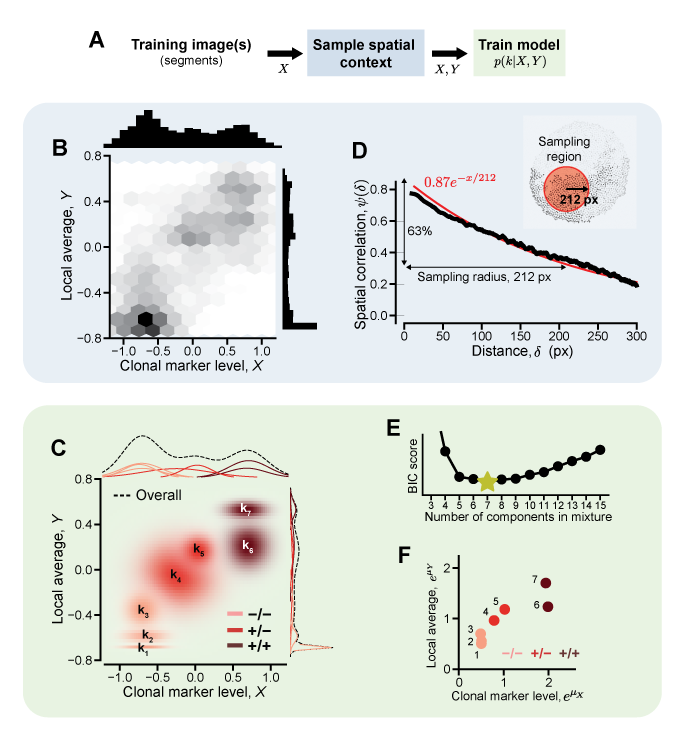
\includegraphics[scale=1.0]{./figure_S3}
\caption[Reductions in energy metabolism limit the extent to which protein expression dynamics are affected by loss of a repressor.]{\textbf{Reductions in energy metabolism limit the extent to which protein expression dynamics are affected by loss of a repressor.} (A-B) Graphical depiction of the method used to quantify the impact of repressor loss on protein expression dynamics. (A) Confidence bands span the 1\textsuperscript{st} to 99\textsuperscript{th} quantiles of protein levels simulated under full repression (grey) and under partial repression (purple), where a repressor is lost. The dashed purple line denotes the lower bound of the purple confidence band. The symbol $\tau$ denotes the commitment time as defined previously. (B) Loss of a repressor causes protein overexpression $E(t)$, which is calculated as the fraction of simulations that exceed the confidence band observed under full repression (grey) at a given time point. Orange-brown color scale reflects the value of $E(t)$ for each time point in the time course. Percent overexpression is calculated as a percent of simulations that exceed the confidence band integrated over the entire time course. A maximum of 100\% overexpression would occur when all simulations exceed the confidence band at all timepoints. (C) Percent overexpression caused by loss of a repressor for model simulations performed with 2500 independent parameter sets. Color scale reflects the strength of overexpression. Overexpression is large for most parameter sets. (D) Percent overexpression caused by loss of a repressor was calculated for simulations implementing normal energy metabolism and reduced energy metabolism. The difference in percent overexpression between the two metabolic conditions is shown for model simulations performed with 2500 independent parameter sets. Color scale reflects the difference. The majority of simulations are blue, indicating that expression dynamics are less affected by repressor loss when energy metabolism is low.}
\label{fig:metabolism:figS3}
\end{figure}

\begin{figure}[h!]
\centering
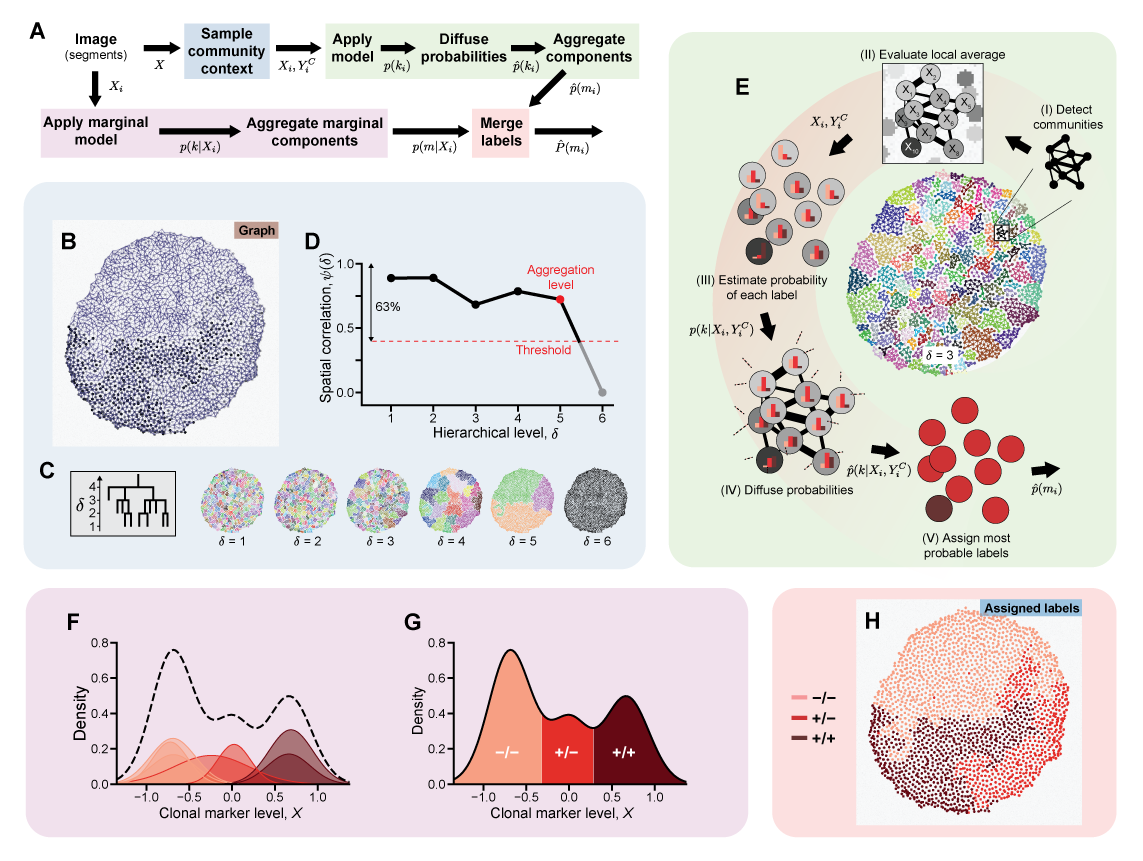
\includegraphics[width=1.0\columnwidth]{./figure_S4}
\caption[Reduced protein synthesis capacity diminishes the importance of auxiliary repression over a wide range of model conditions.]{\textbf{Reduced protein synthesis capacity diminishes the importance of auxiliary repression over a wide range of model conditions.} Each panel depicts a parameter sweep of the nine-dimensional hyperspace defined by one order of magnitude variation in each of the respective model parameters. For each parameter set, error frequency and percent overexpression were calculated as described earlier in Figs. \ref{fig:metabolism:figS2a} and \ref{fig:metabolism:figS3}. They pertain to 50\% reduced repression mimicking auxiliary repressor loss. Error frequency and percent overexpression were calculated independently for conditions of normal and reduced protein synthesis. The difference in error frequency or overexpression between metabolic conditions are shown color-coded, e.g. blue indicates error suppression by reduced protein synthesis. (A-C) Simulations in which the duration of the stimulus input is constant. Shown are the (A) differential error frequencies and (B) differential changes in expression dynamics relative to normal protein synthesis conditions. (C) Differential error frequencies for varying definitions of the success threshold. Each line represents one parameter set, colored by the corresponding range of differential error frequencies. (D) Simulations where a nonzero basal stimulus is applied. (E) Simulations where input duration is increased two-fold by a reduction in protein synthesis capacity. (F) Simulations when an upper bound is placed on the number of sites firing transcription. (G) Simulations when cooperative transcription kinetics are considered.}
\label{fig:metabolism:figS4}
\end{figure}